\subsection{Transportation Economics}
\label{sec:literature:taxis}

Taxis (also known as \textit{taxicabs}) are an important part of public
transportation. Because of their prevalence worldwide and importance in
transportation a wide range of literature has been produced on taxis. For this
project, the most relevant area of these works is economical modelling of taxi
markets, an overview of which is given by \textcite{Salanova2011taxi+review}. A
major topic in the research and discussion on taxis is taxi market regulation,
and parts of it are relevant and will be considered in some detail. Three
different types of taxi markets can be distinguished: cruising taxi market when
a passenger hails the taxi on street with visual contact, phone-order taxi
market, and taxi ranks where multiple taxis wait for passengers.


\subsubsection{Regulation}

Regulation is a controversial topic in taxi market research as no consensus has
been reached on whether it is recommended.
\textcite{Cairns1996taxi+competition} investigated economic workings of taxi
markets and incorporated results of earlier research in their economic
equilibria findings. They concluded that regulation is needed to achieve non-
negative profits (the so-called economic second best).
\textcite{Oecd2007taxi+policy}, cited by \textcite{Salanova2011taxi+review}
listed arguments both for and against regulation as observed in different
countries, and noted that markets with widely varying regulation can operate
successfully. It is important to note that some markets considered
\textit{deregulated} still have some form of fare regulation, for example,
taxis in New Zealand are required to list their maximum fares based on time and
distance, but are not forced to follow them
\parencite{Gaunt1995taxi+newzealand}.


\subsubsection{Economic modelling} 
\label{sec:literature:taxis:modelling}

Taxi market modelling was first done by \textcite{Douglas1972taxi+regulation},
according to \textcite{Salanova2011taxi+review}. He investigated a regulated
cruising-taxi market and defined the fundamental taxi problem to be finding an
equilibrum of an optimal level of service matching an optimal price. His
limited model has been used as reference by all the later authors cited by
\textcite{Salanova2011taxi+review} that have extended it to other taxi markets
and factored in more environmental influences.

\textcite{Devany1975taxi+capacity} researched regulated taxi markets organised
as a franchised monopoly, using a medallion system, and having free entry. With
the goal of finding equilibrium output, capacity and utilisation he suggested a
formula tor passenger demand depending on taxi fare, passenger value of time
and waiting time. \textcite{Manski1967taxi+demand} analysed the taxi market
from a purely economical point of view and conclude that in addition to
exogenous variables, passenger demand for taxi services is also directly
related to taxi supply through waiting time. Similarly, taxi supply is
influenced by taxi utilisation, which in turn directly depends on passenger
demand.

The most recent publications in this area are sophisticated models based on the
network model for cruising-taxi market by \textcite{Yang1998taxi+network}. This
network was modelled as a graph and assumed constant taxi demand and supply,
passenger demand was represented as origin-destination matrices. Finally, this
paper suggested an algorithm to find an equilibrum for the optimal number of
taxis in a market and equations to calculate taxi utilisation and customer
waiting time.

In contrast, \textcite{Yang2000taxi+utilization} focused on supply and demand
to recommend optimal policies for taxi regulation in Hong Kong and based their
model on various data sources. A number of exogenous and endogenous variables
affecting taxi market were identified, and equations were suggested to
calculate them: passenger waiting time, percentage of occupied taxis, vacant
taxi headway, number of daily taxi passenger trips and taxi waiting time. This
model can be used to forecast taxi demand, taxi utilization and service
quality, although the authors warned that it does not take in account all of
the complex supply-demand relationships in taxi market.

Consequently \textcite{Yang2002taxi+demand} continued to evaluate the supply-
demand equilibria of taxi market started by \textcite{Yang1998taxi+network} and
\textcite{Yang2000taxi+utilization}, resulting in the conclusion that the
spatial characteristics of a network where taxis are operating strongly
influence supply and demand, and should bear weight when evaluating regulatory
policies.This study focused on social surplus (the sum of customer surplus and
producer surplus) as the key objective of taxi markets. Four different
regulatory frameworks that could be applied to taxi markets were investigated:
free entry and unconstrained fare, free entry and regulated fare, regulated
entry and unconstrained fare, and regulated entry and regulated fare. All of
these cases were investigated with both competitive and monopilistic markets,
and equilibria were found.

\textcite{Wong2008taxi+modeling} extended this model to heterogenous vehicle
and user classes, and included congestion which is a major issue in reality but
was ignored by earlier research. \textcite{Yang2010taxi+nonlinear} proposed a
nonlinear fare structure to correct market and regulatory inefficiencies, and
applied it to a similar model.

The way how cruising taxis and customers find each other was researched by
\textcite{Yang2010taxi+equilibria}, paying particular attention to customer
behaviour: this study permitted customers to use other modes of transport e.g.
public transit or walking to find taxis and/or reach their destinations.
However, this study was based on a taxi market with fixed fares. When fares can
be negotiated, taxis and customers are likely to do some bargaining over the
amount of fare.

\textcite{Cairns1996taxi+competition} gives a quick overview of bargaining and
its implications in different markets, with customers having more power in taxi
rank and phone order markets due to easily available competition, and high
costs to search for alternatives in cruising taxi market for both parties
resulting in higher willingness to agree. Bargaining of minimal-intelligence
agents in competitive markets was investigated and implemented in software by
\textcite{Cli1997taxi+bargaining}, where a bargaining performance similar to
humans was achieved. \textcite{Rubinstein1982taxi+bargaining} described
equilibria for a bargaining model where each round of barganing has costs to
participants.


\subsubsection{Demand and supply}
\label{sec:literature:taxis:demand}

Taxi demand is a part of the total demand for transportation. There are two
approaches to modelling demand for public transportation: aggregate and
disaggregate. Aggregate models are macroeconomic, while disaggregate models are
microeconomic and based on the individual agents in a system. Recently
disaggregate models have emerged as the main method of modelling demand, but
these models require detailed microeconomic data for a system. Because of
difficult processing of the large datasets, applying disaggregate models
usually still involves some form of aggregation. Customers' value of time (VOT)
and value of reliability (VOR) are the most important quantities determining
the demand for public transportation, the sum of whom are a customer's total
willingness to pay for some trip. Both VOT and VOR derive on customers'
characteristics and environment they are in, for example, their income, whether
the planned trip is for pleasure or a commute to work, and even the tax rates.
Aggregate models using VOT and VOR have been developed as well, although VOR
has been researched significantly less. \parencite{Small2007taxi+urban}

\textcite{Yang2002taxi+demand} cites \textcite{Manski1967taxi+demand} on the
complex structure of demand in taxi markets, shown in Figure~\ref{figure:taxi}.
Both taxi demand and supply are infulenced by exogenous variables (and
regualtion policies, if any). Taxi demand influences taxi availability and vice
versa. Similarly, taxi supply influences taxi utilization and vice versa. Taxi
demand influences taxi utilization and thus indirectly influences supply,
similarly taxi supply influences taxi availability and thus indirectly
influences demand.

\begin{figure}
  \begin{center}
    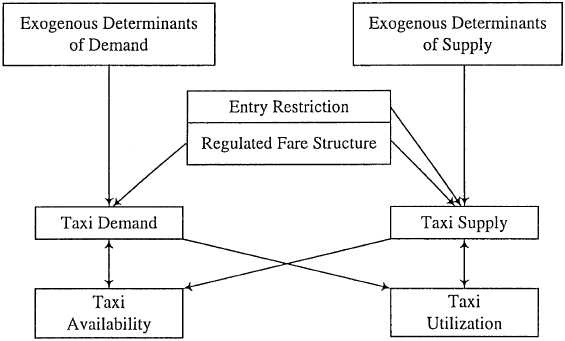
\includegraphics{../figures/taxi_demand}
    \caption{
      Demand-availibility-utilization-supply relation in a taxi market. Manski 
      and Wright (1976), cited by \textcite{Yang2002taxi+demand}.
      \label{figure:taxi}
    }
  \end{center}
\end{figure}

Customer demand is modelled as a function of waiting time and fare price in
many studies: \textcite{Douglas1972taxi+regulation, Devany1975taxi+capacity,
Cairns1996taxi+competition, Yang2002taxi+demand} all used customer waiting time
as a proxy for service quality. According to
\textcite{Salanova2011taxi+review}, \textcite{Manski1967taxi+demand} used a
Poisson process (a stohastic function) to simulate demand.

\textcite{Yang2002taxi+demand} use a disaggregate demand model (separately for
each origin-destination pair), where waiting time depends on the number of
vacant taxis in an area near the customer and price depends on the distance
covered; \textcite{Yang2010taxi+nonlinear} added travel time as an additional
variable indicating service quality and assumed that demand decreases as
waiting time increases. \textcite{Yang2010taxi+equilibria} took a slightly
different approach by modelling customer demand as their willingness to pay to
reach a destination, based on their subjective monetary value for using
different modes of transport for reaching a destination; therefore the demand
for taxis in this study was only a part of the total demand for transportation.
